\documentclass[
  a4paper,
  oneside,
  BCOR = 10mm,
  DIV = 12,
  12pt,
  headings = normal,
]{scrartcl}

%%% Length calculations
\usepackage{calc}
%%%

%%% Support for color
\usepackage{xcolor}
\definecolor{lightblue}{HTML}{03A9F4}
\definecolor{red}{HTML}{F44336}
%%%

%%% Including graphics
\usepackage{graphicx}
%%%

%%% Font selection
\usepackage{fontspec}

\setromanfont{STIX Two Text}[
  SmallCapsFeatures = {LetterSpace = 8},
]

\setsansfont{IBM Plex Sans}[
  Scale = MatchUppercase,
]

\setmonofont{IBM Plex Mono}[
  Scale = MatchUppercase,
]
%%%

%%% Math typesetting
\usepackage{amsmath}
\usepackage{mathtools}

\usepackage{unicode-math}
\setmathfont{STIX Two Math}

\usepackage{IEEEtrantools}
%%%

%%% List settings
\usepackage{enumitem}
\setlist[enumerate]{
  label*      = {\arabic*.},
  left        = \parindent,
  topsep      = 0\baselineskip,
  parsep      = 0\baselineskip,
  noitemsep, % override itemsep
}
% List settings for levels 2–4
\setlist[enumerate, 2, 3, 4]{
  label*      = {\arabic*.},
  left        = 0em,
  topsep      = 0\baselineskip,
  parsep      = 0\baselineskip,
  noitemsep, % override itemsep
}

\setlist[itemize]{
  label*      = {—},
  left        = \parindent,
  topsep      = 0\baselineskip,
  parsep      = 0\baselineskip,
  itemsep     = 1\baselineskip,
  noitemsep, % override itemsep
}

\setlist[description]{
  font        = {\rmfamily\upshape\bfseries},
  topsep      = 1\baselineskip,
  parsep      = 0\baselineskip,
  itemsep     = 0\baselineskip,
}

%%%

%%% Structural elements typesetting
\setkomafont{pagenumber}{\rmfamily\upshape}
\setkomafont{disposition}{\rmfamily\bfseries}

% Sectioning
\RedeclareSectionCommand[
  beforeskip = -1\baselineskip,
  afterskip  = 1\baselineskip,
  font       = {\normalsize\bfseries\scshape},
]{section}

\RedeclareSectionCommand[
  beforeskip = -1\baselineskip,
  afterskip  = 1\baselineskip,
  font       = {\normalsize\bfseries\itshape},
]{subsection}

\RedeclareSectionCommand[
  beforeskip = -1\baselineskip,
  afterskip  = 1\baselineskip,
  font       = {\normalsize\bfseries},
]{subsubsection}

\RedeclareSectionCommand[
  beforeskip = -1\baselineskip,
  afterskip  = -0.5em,
  font       = {\normalsize\mdseries\scshape\addfontfeatures{Letters = {UppercaseSmallCaps}}},
]{paragraph}
%%%

%%% Typographic enhancements
\usepackage{microtype}
%%%

%%% Language-specific settings
\usepackage{polyglossia}
\setmainlanguage{ukrainian}
\setotherlanguages{english}
%%%

%%% Captions
\usepackage{caption}
\usepackage{subcaption}

%\DeclareCaptionLabelFormat{closing}{#2)}
%\captionsetup[subtable]{labelformat = closing}

%\captionsetup[subfigure]{labelformat = closing}

\captionsetup[table]{
  aboveskip = 0\baselineskip,
  belowskip = 0\baselineskip,
}

\captionsetup[figure]{
  aboveskip = 1\baselineskip,
  belowskip = 0\baselineskip,
}

\captionsetup[subfigure]{
  labelformat = simple,
  labelformat = brace,
  justification = RaggedRight,
  singlelinecheck = false,
}
%%%

%%% Hyphenated ragged typesetting
\usepackage{ragged2e}
%%%

%%% Table typesetting
\usepackage{booktabs}
\usepackage{longtable}

\usepackage{multirow}

\usepackage{array}
\newcolumntype{v}[1]{>{\RaggedRight\arraybackslash\hspace{0pt}}p{#1}}
\newcolumntype{b}[1]{>{\Centering\arraybackslash\hspace{0pt}}p{#1}}
\newcolumntype{n}[1]{>{\RaggedLeft\arraybackslash\hspace{0pt}}p{#1}}
%%%

%%% Drawing
\usepackage{tikz}
\usepackage{tikzscale}
\usetikzlibrary{datavisualization}
\usetikzlibrary{datavisualization.formats.functions}
\usetikzlibrary{positioning}
\usetikzlibrary{patterns}
\usetikzlibrary{intersections}
\usetikzlibrary{arrows.meta} % Stealth arrow tips
\usetikzlibrary{graphs}
\usetikzlibrary{graphdrawing}
\usegdlibrary{trees}
\usetikzlibrary{quotes}

\usepackage{pgfplots}
\usepgfplotslibrary{fillbetween}
%%%

%%% SI units typesetting
\usepackage{siunitx}
\sisetup{
  output-decimal-marker = {,},
  exponent-product      = {\cdot},
  inter-unit-product    = \ensuremath{{} \cdot {}},
  per-mode              = symbol,
}
%%%

% Code Highlighting
\usepackage{minted}
\setmintedinline{
  style = bw,
  breaklines,
}

\newminted[bashterm]{text}{%
  autogobble,%
  breaklines,%
  style=bw,%
}

\newminted[codegeneric]{text}{%
  autogobble,%
  style=bw,%
  breaklines,%
  fontsize=\small,%
}

\newmintinline{bash}{%
}

\newmintinline[minttext]{text}{%
  breaklines,%
  breakanywhere,%
}

%%% Framing code listings
\usepackage{tcolorbox}
\tcbuselibrary{breakable}
\tcbuselibrary{minted}
\tcbuselibrary{skins}

% Text file listing
\newtcblisting[
  auto counter,
  list inside,
  number within = section,
]{listingplaintext}[3][]{%
  minted language = text,
  minted style    = bw,
  minted options  = {
    autogobble,
    linenos,
    tabsize = 4,
    breaklines,
    breakanywhere,
    fontsize = \footnotesize,
  },
  empty,
  sharp corners,
  coltitle = black,
  borderline horizontal = {1pt}{0pt}{black},
  titlerule = {0.5pt},
  titlerule style = {
    black,
  },
  toptitle = 0.3em,
  bottomtitle = 0.3em,
  before skip      = \intextsep,
  after  skip      = \intextsep,
  title            = {Лістинг \thetcbcounter: #2},
  list entry       = {\protect\numberline{\thetcbcounter}#2},
  left = 0em,
  right = 0em,
  %
  listing only,
  breakable,
  %
  label = {#3},%
}

\newtcbinputlisting[
  use counter from = listingplaintext,
  list inside,
  number within = section
]{\inputplaintext}[4][]{%
  minted language = text,
  minted style    = bw,
  minted options  = {
    autogobble,
    linenos,
    tabsize = 4,
    breaklines,
    breakanywhere,
    fontsize = \footnotesize,
  },
  empty,
  sharp corners,
  coltitle = black,
  borderline horizontal = {1pt}{0pt}{black},
  titlerule = {0.5pt},
  titlerule style = {
    black,
  },
  toptitle = 0.3em,
  bottomtitle = 0.3em,
  before skip      = \intextsep,
  after  skip      = \intextsep,
  title            = {Лістинг \thetcbcounter: #3},
  list entry       = {\protect\numberline{\thetcbcounter}#3},
  left = 0em,
  right = 0em,
  %
  listing file={#2},
  listing only,
  breakable,
  %
  label = {#4}
}

\newtcblisting[
  use counter from = listingplaintext,
  list inside,
  number within = section,
]{listingpython}[3][]{%
  minted language = python,
  minted style    = bw,
  minted options  = {
    autogobble,
    linenos,
    tabsize = 4,
    breaklines,
    breakanywhere,
    fontsize = \footnotesize,
  },
  empty,
  sharp corners,
  coltitle = black,
  borderline horizontal = {1pt}{0pt}{black},
  titlerule = {0.5pt},
  titlerule style = {
    black,
  },
  toptitle = 0.3em,
  bottomtitle = 0.3em,
  before skip      = \intextsep,
  after  skip      = \intextsep,
  title            = {Лістинг \thetcbcounter: #2},
  list entry       = {\protect\numberline{\thetcbcounter}#2},
  left = 0em,
  right = 0em,
  %
  listing only,
  breakable,
  %
  label = {#3},
  %
  #1%
}

\newtcbinputlisting[
  use counter from = listingplaintext,
  list inside,
  number within = section
]{\inputpython}[4][]{%
  minted language = python,
  minted style    = bw,
  minted options  = {
    autogobble,
    linenos,
    tabsize = 4,
    breaklines,
    breakanywhere,
    fontsize = \footnotesize,
  },
  empty,
  sharp corners,
  coltitle = black,
  borderline horizontal = {1pt}{0pt}{black},
  titlerule = {0.5pt},
  titlerule style = {
    black,
  },
  toptitle = 0.3em,
  bottomtitle = 0.3em,
  before skip      = \intextsep,
  after  skip      = \intextsep,
  title            = {Лістинг \thetcbcounter: #3},
  list entry       = {\protect\numberline{\thetcbcounter}#3},
  left = 0em,
  right = 0em,
  %
  listing file={#2},
  listing only,
  breakable,
  %
  label = {#4}
}

% Linux command-line listing
\newtcblisting{linuxterm}%
{%
  % Syntax highlighing options
  listing only,%
  minted language = bash,%
  minted options={%
    autogobble,%
    linenos%
  },%
  % Presentation options
  empty,%
  %% Margins
  sharp corners,%
  toptitle = 0.0em,%
  bottomtitle = 0.0em,%
  left = 0em,%
  right = 0em,%
  before skip = \intextsep,%
  after skip = \intextsep,%
}

\newtcblisting{linuxtermout}%
{%
  % Syntax highlighing options
  listing only,%
  minted language = text,%
  minted options={%
    autogobble,%
    linenos%
  },%
  % Presentation options
  empty,%
  %% Margins
  sharp corners,%
  toptitle = 0.0em,%
  bottomtitle = 0.0em,%
  left = 0em,%
  right = 0em,%
  before skip = \intextsep,%
  after skip = \intextsep,%
}

% Dockerfile listings
\newtcblisting[
  use counter from = listingplaintext,
  list inside,
  number within = section,
]{listingdocker}[3][]{%
  minted language = dockerfile,
  minted style    = bw,
  minted options  = {
    autogobble,%
    linenos,
    tabsize = 4,
    breaklines,
    breakanywhere,
    fontsize = \footnotesize,
  },
  empty,
  sharp corners,
  coltitle = black,
  borderline horizontal = {1pt}{0pt}{black},
  titlerule = {0.5pt},
  titlerule style = {
    black,
  },
  toptitle = 0.3em,
  bottomtitle = 0.3em,
  before skip      = \intextsep,
  after  skip      = \intextsep,
  title            = {Лістинг \thetcbcounter: #2},
  list entry       = {\protect\numberline{\thetcbcounter}#2},
  left = 0em,
  right = 0em,
  %
  listing only,
  breakable,
  %
  label = {#3},%
}

% Docker Compose listings
\newtcblisting[
  use counter from = listingplaintext,
  list inside,
  number within = section,
]{listingdockercompose}[3][]{%
  minted language = yaml,
  minted style    = bw,
  minted options  = {
    autogobble,%
    linenos,
    tabsize = 4,
    breaklines,
    breakanywhere,
    fontsize = \footnotesize,
  },
  empty,
  sharp corners,
  coltitle = black,
  borderline horizontal = {1pt}{0pt}{black},
  titlerule = {0.5pt},
  titlerule style = {
    black,
  },
  toptitle = 0.3em,
  bottomtitle = 0.3em,
  before skip      = \intextsep,
  after  skip      = \intextsep,
  title            = {Лістинг \thetcbcounter: #2},
  list entry       = {\protect\numberline{\thetcbcounter}#2},
  left = 0em,
  right = 0em,
  %
  listing only,
  breakable,
  %
  label = {#3},%
}


% Customize minted line numbers
\renewcommand{\theFancyVerbLine}{\ttfamily\scriptsize\arabic{FancyVerbLine}}

%%%

%%% Typeset menus and keys
\usepackage{menukeys}[
  os=win,
]
%%%

%%% Links and hyperreferences
\usepackage{hyperref}
\hypersetup{
  bookmarksnumbered = true,
  colorlinks      = false,
  linkbordercolor = red,
  urlbordercolor  = lightblue,
  pdfborderstyle  = {/S/U/W 1.5},
}
%%%

%%% Length adjustment

% Set baselineskip, default is 14.5 pt
\linespread{1.068966} % ~15.5 pt
\setlength{\emergencystretch}{1em}
\setlength{\parindent}{1.5em}
\newlength{\gridunitwidth}
\setlength{\gridunitwidth}{\textwidth / 12}
%%%

%%% Custom commands
\newcommand{\allcaps}[1]{%
  {%
    \addfontfeatures{%
      Letters = UppercaseSmallCaps,
      LetterSpace = 8,%
    }%
    #1%
  }%
}
\newcommand{\filename}[1]{\texttt{#1}}
\newcommand{\progname}[1]{\texttt{#1}}
\newcommand{\commandname}[1]{\texttt{#1}}
\newcommand{\modulename}[1]{\texttt{#1}}
\newcommand{\transeng}[1]{{англ.}~\textit{\textenglish{#1}}}
%%%

%%% Custom math commands
\newcommand{\longvar}[1]{\mathit{#1}}
\newcommand{\vect}[1]{\mathbfit{#1}}
\newcommand{\matr}[1]{\mathbfit{#1}}

\newcommand{\logequiv}{\mathrel{\Longleftrightarrow}} % Logically equivalent

\newcommand{\ssep}{\mid} % set builder separator

\DeclareMathOperator*{\minimize}{min} % minimize for linear programs
\DeclareMathOperator*{\rand}{rand} % rand()

\DeclarePairedDelimiter{\setpower}{\lvert}{\rvert} % set power
%%%

\begin{document}

\begin{titlepage}
    \begin{center}
      Міністерство освіти і~науки України\\
      Національний авіаційний університет\\
      Факультет кібербезпеки, комп'ютерної та~програмної інженерії\\
      Кафедра комп'ютеризованих систем управління

      \vspace{\fill}
        Лабораторна робота №~3.4\\
        з~дисципліни «Технології проектування комп'ютерних систем»\\
        на~тему «Моделювання одноканальної системи обслуговування методом статистичного моделювання»

      \vspace{\fill}

      \begin{flushright}
        Виконав:\\
        студент \allcaps{ФККПІ}\\
        групи \allcaps{СП}-425\\
        Клокун В.\,Д.\\
        Перевірила:\\
        Голего Н.\,М.
      \end{flushright}

      Київ 2020
    \end{center}
  \end{titlepage}

  \section{Мета роботи}
    Провести моделювання функціонування системи масового обслуговування та~визначити показники її~роботи.

  \section{Хід~роботи}
    Створюємо 2~множини: множину тривалостей часу з~моменту закінчення обробки попередньої заявки до~моменту надходження наступної заявки~$T_i$ та~множину тривалостей обслуговування $i$-ї~заявки~$T_{\text{обсл}}$. Кожна множина повинна складатись з~$n = 10$~рівномірно розподілених випадкових чисел. Також, елементи кожної з~множин повинні задовольняти таким умовам: $t_i \in [0; K)$, $t_{\text{обсл}} \in [0; L)$, де~$K = 13$, $L = 8$ за~умовами варіанту.

    Отже, математично необхідні множини можна записати так:
    \begin{IEEEeqnarray*}{rCl}
      T_i &=& \left\{
        t_i \ssep
        t_i = \rand(), \,
        t_i \in [0, K), \,
        \setpower{T_i} = 10
      \right\} \\
    T_{\text{обсл}} &=& \left\{
        t_{\text{обсл}} \ssep
        t_{\text{обсл}} = \rand(), \,
        t_{\text{обсл}} \in [0, L), \,
        \setpower{T_{\text{обсл}}} = 10
      \right\}
    \end{IEEEeqnarray*}
    В~результаті отримали необхідні множини~(табл.~\ref{tab:input-vals}).

    \begin{table}[!htbp]
      \caption{Вхідні дані}
      \label{tab:input-vals}
      \begin{tabular}{
        v{2\gridunitwidth - 2\tabcolsep}
        *{10}{n{1\gridunitwidth - 2\tabcolsep}}
      }
        \toprule
          № заявки & 1 & 2 & 3 & 4 & 5 & 6 & 7 & 8 & 9 & 10 \\
        \midrule
          $t_{i}$             & 2 & 0 & 5 & 4 & 2 & 4 & 3 & 3 & 3 & 0 \\
          $t_{\text{обсл}}$ & 2 & 2 & 3 & 2 & 3 & 0 & 3 & 0 & 0 & 0 \\
        \bottomrule
      \end{tabular}
    \end{table}

    Моделюємо роботу системи та~відкладаємо отримані вхідні дані на~осі~часу~$t$~(рис.~\ref{fig:system-model-time-diag}).

    \begin{figure}[!htbp]
      \centering
      \small
      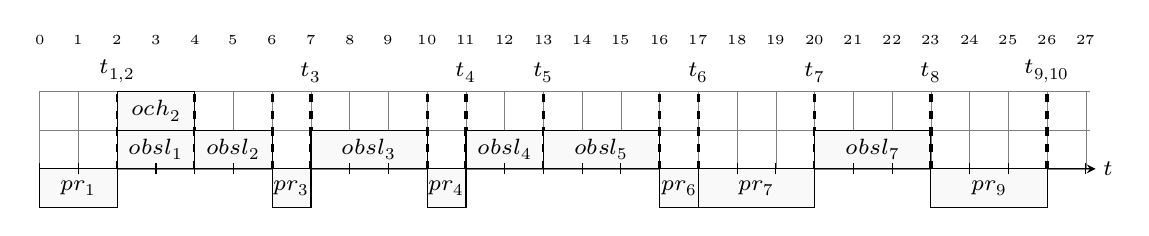
\begin{tikzpicture}[x = 1.4em, y = 1.4em]
        \footnotesize
        \draw[help lines, step=1] (0.0, 0.0) grid (27.1, 2.0);

        % Coordinate lines
        \begin{scope}[>=stealth]
          \draw[->] (0, 0) -- (27.25, 0) node[right] {$t$};
          % \draw[->] (0, 0) -- (0, 4)   node[above] {$N$};
        \end{scope}

        \begin{scope}
          % step 01
          %
          \draw [fill = black!2.5]
            (00,  00) rectangle node {$pr_1$} (02, -01);
          \draw [dashed, very thick]
            (02,  00) -- (02,  02) node [anchor = south] {$t_{1, 2}$};

          % step 02
          %
          \draw [fill = black!2.5]
            (02,  00) rectangle node {$obsl_1$} (04, +01);
          \draw [fill = black!2.5]
            (02,  01) rectangle node {$och_2$} (04, +02);
          \draw [dashed, very thick]
            (04,  00) -- (04,  02);

          % step 03
          %
          \draw [fill = black!2.5]
            (04,  00) rectangle node {$obsl_2$} (06, +01);
          \draw [dashed, very thick]
            (06,  00) -- (06,  02);

          % step 04
          %
          \draw [fill = black!2.5]
            (06,  00) rectangle node {$pr_3$} (07, -01);
          \draw [dashed, very thick]
            (07,  00) -- (07,  02) node [anchor = south] {$t_{3}$};

          % step 05
          %
          \draw [fill = black!2.5]
            (07,  00) rectangle node {$obsl_3$} (10, +01);
          \draw [dashed, very thick]
            (10,  00) -- (10,  02);

          % step 06
          %
          \draw [fill = black!2.5]
            (10,  00) rectangle node {$pr_4$} (11, -01);
          \draw [dashed, very thick]
            (11,  00) -- (11,  02) node [anchor = south] {$t_{4}$};

          % step 07
          %
          \draw [fill = black!2.5]
            (11,  00) rectangle node {$obsl_4$} (13, +01);
          \draw [dashed, very thick]
            (13,  00) -- (13,  02) node [anchor = south] {$t_{5}$};

          % step 08
          %
          \draw [fill = black!2.5]
            (13,  00) rectangle node {$obsl_5$} (16, +01);
          \draw [dashed, very thick]
            (16,  00) -- (16,  02);

          % step 09
          %
          \draw [fill = black!2.5]
            (16,  00) rectangle node {$pr_6$} (17, -01);
          \draw [dashed, very thick]
            (17,  00) -- (17,  02) node [anchor = south] {$t_{6}$};

          % step 10
          %
          \draw [fill = black!2.5]
            (17,  00) rectangle node {$pr_7$} (20, -01);
          \draw [dashed, very thick]
            (20,  00) -- (20,  02) node [anchor = south] {$t_{7}$};

          % step 11
          %
          \draw [fill = black!2.5]
            (20,  00) rectangle node {$obsl_7$} (23, +01);
          \draw [dashed, very thick]
            (23,  00) -- (23,  02) node [anchor = south] {$t_8$};

          % step 12
          %
          \draw [fill = black!2.5]
            (23,  00) rectangle node {$pr_{9}$} (26, -01);
          \draw [dashed, very thick]
            (26,  00) -- (26,  02) node [anchor = south] {$t_{9, 10}$};
        \end{scope}

        \newcommand*{\TickSize}{0.25em}
        % x ticks
        \begin{scope}
          \foreach \x in {0,...,27} {%
            \draw ($(\x,0) + (0,-\TickSize)$) -- ($(\x,0) + (0,\TickSize)$)
            node [anchor = north, above = 5em, font={\tiny}] {$\x$};
            }
        \end{scope}
        % y ticks
        % \begin{scope}
        %   \foreach \y in {0,...,3} {%
        %       \draw ($(0,\y) + (-\TickSize,0)$) -- ($(0,\y) + (\TickSize,0)$)
        %           node [anchor = east, left = 1em] {CPU $\y$};
        %   }
        % \end{scope}

        % \begin{scope}
        %   \foreach \y in {0,...,2} {%
        %     \node[anchor = east] at (0, \y + 0.5) {$\y$};
        %     }
        % \end{scope}
      \end{tikzpicture}
      \caption{Часова діаграма обслуговування заявок}
      \label{fig:system-model-time-diag}
    \end{figure}

    За~часовою діаграмою роботи системи знаходимо характеристики кожної заявки, що~нас~цікавлять~(табл.~\ref{tab:system-ticket-performance}).

    \begin{table}[!htbp]
      \caption{Характеристики заявок у~системі}
      \label{tab:system-ticket-performance}
      \begin{tabular}{
        v{2 \gridunitwidth - 2\tabcolsep}
        *{10}{n{1 \gridunitwidth - 2\tabcolsep}}
      }
        \toprule
          № заявки          & 1 & 2 & 3 & 4 & 5 & 6 & 7 & 8 & 9 & 10 \\
        \midrule
          $\textit{pr}_i$   & 2 & 0 & 1 & 1 & 0 & 0 & 3 & 0 & 3 & 0 \\
          $\textit{obsl}_i$ & 2 & 2 & 3 & 2 & 3 & 0 & 3 & 0 & 0 & 0 \\
          $\textit{och}_i$  & 0 & 2 & 0 & 0 & 0 & 0 & 0 & 0 & 0 & 0 \\
          $\textit{dovj}_i$ & 1 & 0 & 0 & 0 & 0 & 0 & 0 & 0 & 0 & 0 \\
        \bottomrule
      \end{tabular}
    \end{table}

    Знаходимо середній час~очікування заявки у~системі~$\textit{och}_{\text{ser}}$:
    \begin{IEEEeqnarray*}{rCl}
      \textit{och}_\text{ser} &=&
      \frac{1}{n} \sum_{i = 1}^{n} \textit{och}_i
      =  \frac{0 + 2 + 0 + 0 + 0 + 0 + 0 + 0 + 0 + 0}{10}
      =  \frac{2}{10} = \num{0,2}.
    \end{IEEEeqnarray*}
    Знаходимо середню довжину черги у~системі~$\textit{dovj}_{\text{ser}}$:
    \begin{IEEEeqnarray*}{rCl}
      \textit{dovj}_\text{ser} &=&
      \frac{1}{n} \sum_{i = 1}^{n} \textit{dovj}_i
      = \frac{1 + 0 + 0 + 0 + 0 + 0 + 0 + 0 + 0 + 0}{10}
      = \frac{1}{10} = \num{0,1}.
    \end{IEEEeqnarray*}
    З~часової діаграми визначаємо тривалість моделювання~$t_{\text{mod}}$ і~знаходимо ймовірність простою каналу у~системі:
    \begin{IEEEeqnarray*}{rCl}
      P_\text{pr} &=& \frac{1}{t_\text{mod}} \sum_{i = 1}^{n} pr_i
                   = \frac{2 + 0 + 1 + 1 + 0 + 0 + 3 + 0 + 3 + 0}{26}
                   = \frac{10}{26} = \frac{5}{13}.
    \end{IEEEeqnarray*}
    Знаходимо ймовірність зайнятості каналу~$P_z$:
    \begin{IEEEeqnarray*}{rCl}
      P_\text{z} &=& 1 - P_\text{pr} = 1 - \frac{5}{13} = \frac{8}{13}.
    \end{IEEEeqnarray*}
    Отже, ми~визначили, що~у~системі середній час~очікування заявки ~$\textit{och}_\text{ser} = \num{0,2}$, середня довжина черги~$\textit{dovj}_\text{ser} = \num{0,1}$, ймовірність простою~$P_\text{pr} = 5/13$, ймовірність зайнятості каналу~$P_\text{z} = 8/13$.

  \section{Висновок}
    Виконуючи дану лабораторну роботу, ми~провели моделювання функціонування системи масового обслуговування та~визначили показники її~роботи.

\end{document}
